\section{Un po' più di geometria (simplettica)}
\setcounter{equation}{0}
Riepilogo della formulazione lagrangiana della meccanica classica \\

\begin{center}
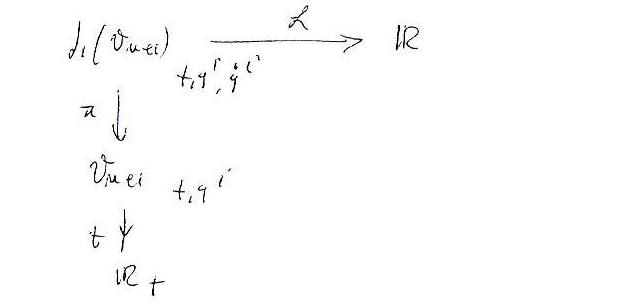
\includegraphics[width=0.5\columnwidth]{media/un-po-di-geometria-simplettica/18-1.jpg}
\end{center}

$ t, q^i $ coordinate fibrate su $\mathcal{V}_{n+1}$, spazio tempo degli eventi in presenza di vincoli \\

$ t, q^i, \dot{q}^i $ coordinate naturali in $j_1 (\mathcal{V}_{n+1})$, spazio tempo degli stati cinetici in presenza di vincoli. \\

\begin{equation*}
\begin{cases}
t' = t \\
q'^i = q'^i (t, q)
\end{cases}
\end{equation*}

\begin{center}
gruppo di trasformazione di coordinate in $\mathcal{V}_{n+1}$
\end{center}

\begin{equation*}
\begin{cases}
t' = t \\
q'^i = q'^i (t, q) \\
\dot{q}'^i = \frac{\partial q'^i}{\partial t} (t, q) + \frac{\partial q'^i}{\partial q^k} (t, q) \dot{q}^k
\end{cases}
\end{equation*}

\begin{center}
gruppo di trasfomazioni tra coordinate naturali di $j_1 (\mathcal{V}_{n+1})$
\end{center}

\begin{equation*}
\frac{d}{dt} \frac{\partial \Lagr}{\partial \dot{q}^k} - \frac{\partial \Lagr}{\partial q^k}
\end{equation*}

equazioni di Lagrange \\

\begin{align*}
&\Rightarrow \ddot{q}^k = \ddot{q}^k (t, q, \dot{q}) \overset{\underset{\mathrm{def}}{}}{=} Z^k (t, q, \dot{q}) \\
&\Rightarrow Z = \frac{\partial}{\partial t} + \dot{q}^k \frac{\partial}{\partial q^k} + Z^k (t, q, \dot{q}) \frac{\partial}{\partial \dot{q}^k}
\end{align*}

Nota: $ \Lagr' = \Lagr + \frac{d}{dt} f (t, q) $ e $ \Lagr $ determinano la stessa dinamica (gauge Lagrangiano). \\

\subsubsection*{Esercizio:}

\begin{align*}
\frac{\partial \Lagr}{\partial q^k} &= \frac{\partial \Lagr}{\partial q'^i} \frac{\partial q'^i}{\partial q^k} + \frac{\partial \Lagr}{\partial \dot{q}'^i} \frac{\partial \dot{q}'^i}{\partial q^k}
\\
\frac{\partial \Lagr}{\partial \dot{q}^k} &= \frac{\partial \Lagr}{\partial \dot{q}'^i} \frac{\partial \dot{q}'^i}{\partial \dot{q}^k} = \frac{\partial \Lagr}{\partial \dot{q}'^i} \frac{\partial q'^i}{\partial q^k}
\\
\frac{d}{dt} \frac{\partial \Lagr}{\partial \dot{q}^k} &= \left( \frac{d}{dt} \frac{\partial \Lagr}{\partial \dot{q}'^i} \right) \frac{\partial q'^i}{\partial q^k} + \frac{\partial \Lagr}{\partial \dot{q}'^i} \frac{d}{dt} \frac{\partial q'^i}{\partial q^k}
\\
&= \left( \frac{d}{dt} \frac{\partial \Lagr}{\partial \dot{q}'^i} \right) \frac{\partial q'^i}{\partial q^k} + \frac{\partial \Lagr}{\partial \dot{q}'^i} \frac{\partial \dot{q}'^i}{\partial q^k}
\end{align*}

\begin{equation*}
\Rightarrow \frac{d}{dt} \frac{\partial \Lagr}{\partial \dot{q}^k} - \frac{\partial \Lagr}{\partial q^k} = \left( \frac{d}{dt} \frac{\partial \Lagr}{\partial \dot{q}'^i} - \frac{\partial \Lagr}{\partial q'^i} \right) \frac{\partial q'^i}{\partial q^k}
\end{equation*}

Risulta pertanto mostrata l'invarianza delle equazioni di Lagrange al variare delle \textit{coordinate} in $\mathcal{V}_{n+1}$. \\

Posto $\omega^k = dq^k - \dot{q}^k dt$, un semplice calcolo mostra che

\begin{equation*}
\begin{split}
\omega'^i &= dq^k - \dot{q}'^i dt = \frac{\partial q'^i}{\partial q^k} (dq^k - \dot{q}^k dt) \\
&= \frac{\partial q'^i}{\de q^k} \omega^k
\end{split}
\end{equation*}

Pertanto le equazioni di Lagrange si possono scrivere in forma \textit{vettoriale} nel modo seguente:
\begin{equation*}
\sum_{k=1} ^{N} \left( \frac{d}{dt} \frac{\partial \Lagr}{\partial \dot{q}^k} - \frac{\partial \Lagr}{\partial q^k} \right) \omega^k = 0
\end{equation*}

Similmente, posto $\quad \mathcal{T}_{k|I} = \frac{d}{dt} \frac{\partial T_I}{\partial \dot{q}^k} - \frac{\partial T_I}{\partial q^k}\quad$ e $\quad Q_{k|I} = \sum_{i=1}^{N} F_{i|I} \cdot \frac{\partial P_i}{\partial q^k}$, si può scrivere:

\begin{equation*}
\sum_{k=1}^{N} \mathcal{T}_{k|I} \quad \omega ^k = \sum_{k=1}^{N} Q_{k|I} \quad \omega^k
\end{equation*}

% INIZIO PAGINA 19

\begin{equation*}
H = \frac{\partial \Lagr}{\partial \dot{q}^k}\dot{q}^k - \Lagr = \frac{\partial \Lagr}{\partial \dot{q}^i}\frac{\partial q'^i}{\partial q^k}\dot{q}^k - \Lagr
= \frac{\partial \Lagr}{\partial \dot{q}^i}\left(\dot{q}'^i - \frac{\partial q^i}{\partial t}\right) - \Lagr = H' - \frac{\partial \Lagr}{\partial \dot{q}^i}\frac{\partial q^i}{\partial t}
\end{equation*}

che mostra le leggi di trasformazione della \textit{funzione} Hamiltoniana al variare delle coordinate. \textit{Notare che} $H$ \textit{non è invariante per trasformazioni di coordinate restanti in} $j_1(\mathcal{V}_{n+1})$. \\

Osserviamo inoltre che

\begin{equation*}
\begin{aligned}
- H dt + \frac{\partial \Lagr}{\partial \dot{q}^k} q^k
&= - \left(H' - \frac{\partial \Lagr}{\partial \dot{q}^i}\frac{\partial q'^i}{\partial t}\right)dt + \frac{\partial \Lagr}{\partial \dot{q}^i}\frac{\partial q'^i}{\partial q^k} dq^k \\
&= -H'dt + \frac{\partial \Lagr}{\partial \dot{q}'^i} dq'^i
\end{aligned}
\end{equation*}

La quale mostra che la $ 1 $-forma differenziale, detta di Poincaré-Cartan,

\begin{equation*}
\theta_{\Lagr} = - H dt + \frac{\partial \Lagr}{\partial \dot{q}^k} dq^k
\end{equation*}

ha comportamento \textit{invariantivo} al cambiare delle coordinate. \\

Sotto una trasformazione di gauge $ \Lagr \rightarrow \Lagr' = \Lagr + \frac{df}{dt} $,

\begin{equation*}
\begin{aligned}
\theta_{\Lagr}
&= - H dt + \frac{\partial \Lagr}{\partial \dot{q}^k} dq^k = - \left (\frac{\partial \Lagr}{\partial \dot{q^k}}\dot{q^k} - \Lagr \right) dt + \frac{\partial \Lagr}{\partial \dot{q}^k} q^k \\
&= \Lagr dt + \frac{\partial \Lagr}{\partial \dot{q}^k} \left( dq^k - \dot{q^k} dt \right) = \Lagr dt + \frac{\partial \Lagr}{\partial \dot{q^k}}\omega^k
\end{aligned}
\end{equation*}
diventa
\begin{equation*}
\begin{aligned}
\theta'_{\Lagr} 
&= \left( \Lagr + \frac{df}{dt} \right) dt + \frac{\partial}{\partial \dot{q}^k} \left( \Lagr + \frac{df}{dt} \right) \left(dq^k - \dot{q^k} dt \right) \\
&= \Lagr dt + \frac{\partial f}{\partial t} dt + \frac{\partial \Lagr}{\partial \dot{q^k}}\omega^k + \frac{\partial f}{\partial q^k} \left(dq^k - \dot{q^k} dt\right) \\
&= \left( \Lagr dt + \frac{\partial \Lagr}{\partial \dot{q^k}}\omega^k \right) + \left( \frac{\partial f}{\partial t} dt + \cancel{\frac{\partial f}{\partial q^k} \dot{q^k}} \right) dt + \frac{\partial f}{\partial q^k} \left(dq^k - \cancel{\dot{q^k} dt}\right) \\
&= \theta_{\Lagr} + \frac{\partial f}{\partial t} dt + \frac{\partial f}{\partial q^k} dq^k = \theta_{\Lagr} + df
\end{aligned}
\end{equation*}

I calcoli come svolti mostrano che la $ 1 $-forma differenziale $ \theta_{\Lagr} = - H (t, q, \dot{q}) dt + \frac{\partial \Lagr}{\partial \dot{q^k}} (t, q, \dot{q}) dq^k $ sullo spazio $ j_1 (\mathcal{V}_{n+1}) $, detta $ 1 $-forma di Poincaré-Cartan associata a $ \Lagr $, è un oggetto importante. \\
La si incontrerà molte volte nelle pagine seguenti.
